\documentclass[12pt]{article}

%***************************************************************************************************
% Math
\usepackage{fancyhdr} 
\usepackage{amsfonts}
\usepackage{amsmath}
\usepackage{amssymb}
\usepackage{amsthm}
%\usepackage{dsfont}

%***************************************************************************************************
% Macros
\usepackage{calc}

%***************************************************************************************************
% Commands and Custom Variables	
\newcommand{\problem}[1]{\hspace{-4 ex} \large \textbf{Problem #1} }
\let\oldemptyset\emptyset
\let\emptyset\varnothing
\newcommand{\norm}[1]{\left\lVert#1\right\rVert}
\newcommand{\sint}{\text{s}\kern-5pt\int}
\newcommand{\powerset}{\mathcal{P}}
\renewenvironment{proof}{\hspace{-4 ex} \emph{Proof}:}{\qed}
\newcommand{\RR}{\mathbb{R}}
\newcommand{\NN}{\mathbb{N}}
\newcommand{\QQ}{\mathbb{Q}}
\newcommand{\ZZ}{\mathbb{Z}}
\newcommand{\CC}{\mathbb{C}}

\let\vec\mathbf


%***************************************************************************************************
%page
\usepackage[margin=1in]{geometry}
\usepackage{setspace}
%\doublespacing
\allowdisplaybreaks
\pagestyle{fancy}
\fancyhf{}
\rhead{Shaw \space \thepage}
%\setlength\parindent{0pt}

%***************************************************************************************************
%Code
\usepackage{listings}
\usepackage{courier}
\lstset{
	language=Python,
	showstringspaces=false,
	formfeed=newpage,
	tabsize=4,
	commentstyle=\itshape,
	basicstyle=\ttfamily,
}

%***************************************************************************************************
%Images
\usepackage{graphicx}
\graphicspath{ {images/} }
\usepackage{float}


\title{Progress Report}
\author{Student: Sage Shaw}
\date{April 16, 2018}

%\renewcommand{\abstractname}{Overview}

\usepackage[backend=bibtex, style=numeric, sorting=none]{biblatex}
\addbibresource{pre-proposal.bib}
%\bibliography{SRF}


\begin{document}
	\thispagestyle{empty}
	
	\begin{flushright}
		Sage Shaw \\
		m566 - Spring 2018 \\
		\today
	\end{flushright}
	
	%{\large \textbf{Pre-Proposal}}\bigbreak
	\begin{center}
		\Huge \textbf{Project Proposal} \\
		\large Solving PDEs using RBF-FD in Parallel
	\end{center}

In short, I'm a little behind but still in good shape. Some issues with sparse matrix formats in Python took a very long time to debug but now I have a working implementation of RBF-FD using polyharmonic spline RBFs in serial. I'll be getting scaling results just as soon as I find a few examples of steady-state heat solutions on a disk which shouldn't take too long.

The parallelization has had some design challenges. Parallelizing the formulation of the differentiation matrix still looks simple, but solving the system in parallel has proven more challenging. Serial methods such as BiCGSTAB with an Incomplete LU decomposition preconditioner or GMRES seem to work well.

\section{Timeline}
	The revised timeline in the original proposal is still the goal. With the exceptions of implementing the algorithms in parallel and generating error plots I am on schedule. I am ahead in the sense that the PHS implementation was expected to be finished this week but is already finished. 
	
	By the end of this week I will have generated error plots and started to write about accuracy and stability of RBF-FD with PHS compared with both classical finite difference methods and RBF-FD using a shape parameter. 
	
	\begin{table}[hb]
		\begin{tabular}{ c| p{12cm}} 
			Week 13 & Implement RBF-FD with stencils on a disk in serial and in parallel. Compare accuracy with other numerical techniques.\\
			& \\
			Week 14 & Progress report due. Implement RBF-FD with stencils on a disk using PHS RBF with polynomial basis terms in serial and in parallel. Compare accuracy with other numerical techniques. Assess stability. \\
			&\\
			Week 15 & Implement in C using MPI. Produce scaling results. Presentation due.\\
			&\\
			Time permitting & Implement on GPU. Explore alternative domain decompositions. Reduce memory footprint.\\
			Finals week & Report due.
		\end{tabular}
		\caption{Original Timeline}
	\end{table}
	
%%%%%%%%%%%%%%%%%%%%%%%%%%%%%%%%%%%%%%%%%%%%%%%%%%%%%%%%%%%%%%%%%%%%%%%%%%%%
%%%%%%%%%%%%%%%%%%%%%%%%%%%%%%%%%%%%%%%%%%%%%%%%%%%%%%%%%%%%%%%%%%%%%%%%%%%%
%%%%%%%%%%%%%%%%%%%%%%%%%%%%%%%%%%%%%%%%%%%%%%%%%%%%%%%%%%%%%%%%%%%%%%%%%%%%
	
\section{Parallelization Challenges}
	While I haven't coded the algorithm in parallel I have have a good outline and almost all of the theory worked out. The missing step is the choice of solver. The only difficulty is finding one that will be easy to parallelize in the time provided. 
	
	Otherwise I have made excellent progress. I've thought through the difficulties of doing quick matrix-vector multiplications in parallel and the dot product in parallel. 
	
\subsection{Matrix-Vector Multiplication \& Point Ordering}
	The parallel solvers I am familiar with rely on the ability to do quick matrix vector multiplication. Generally this is done by partitioning the rows of the matrix and vector among the processes operating on them. Consider the matrix with the sparsity pattern indicated on the left in figure \ref{matrix_spy}. If this matrix were to be distributed over two processes the first process would be allocated the first ten rows and the second process would be allocated the remaining ten rows. If we were to multiply this matrix with a vector the first process would need to know all but the last two entries in the vector. If we instead consider the same matrix reordered using the reverse-Cuthill-McKee ordering as seen on the right in figure \ref{matrix_spy} we can see that the first process needs only the first ten values in the vector (which it is expected to have) and only four of the next ten values which will need to be transmitted from the second process.
	
	\begin{figure}[ht]
		\centering
		\begin{tabular}{cc}
			\includegraphics[width=.4\textwidth]{no_order_spy.eps} & 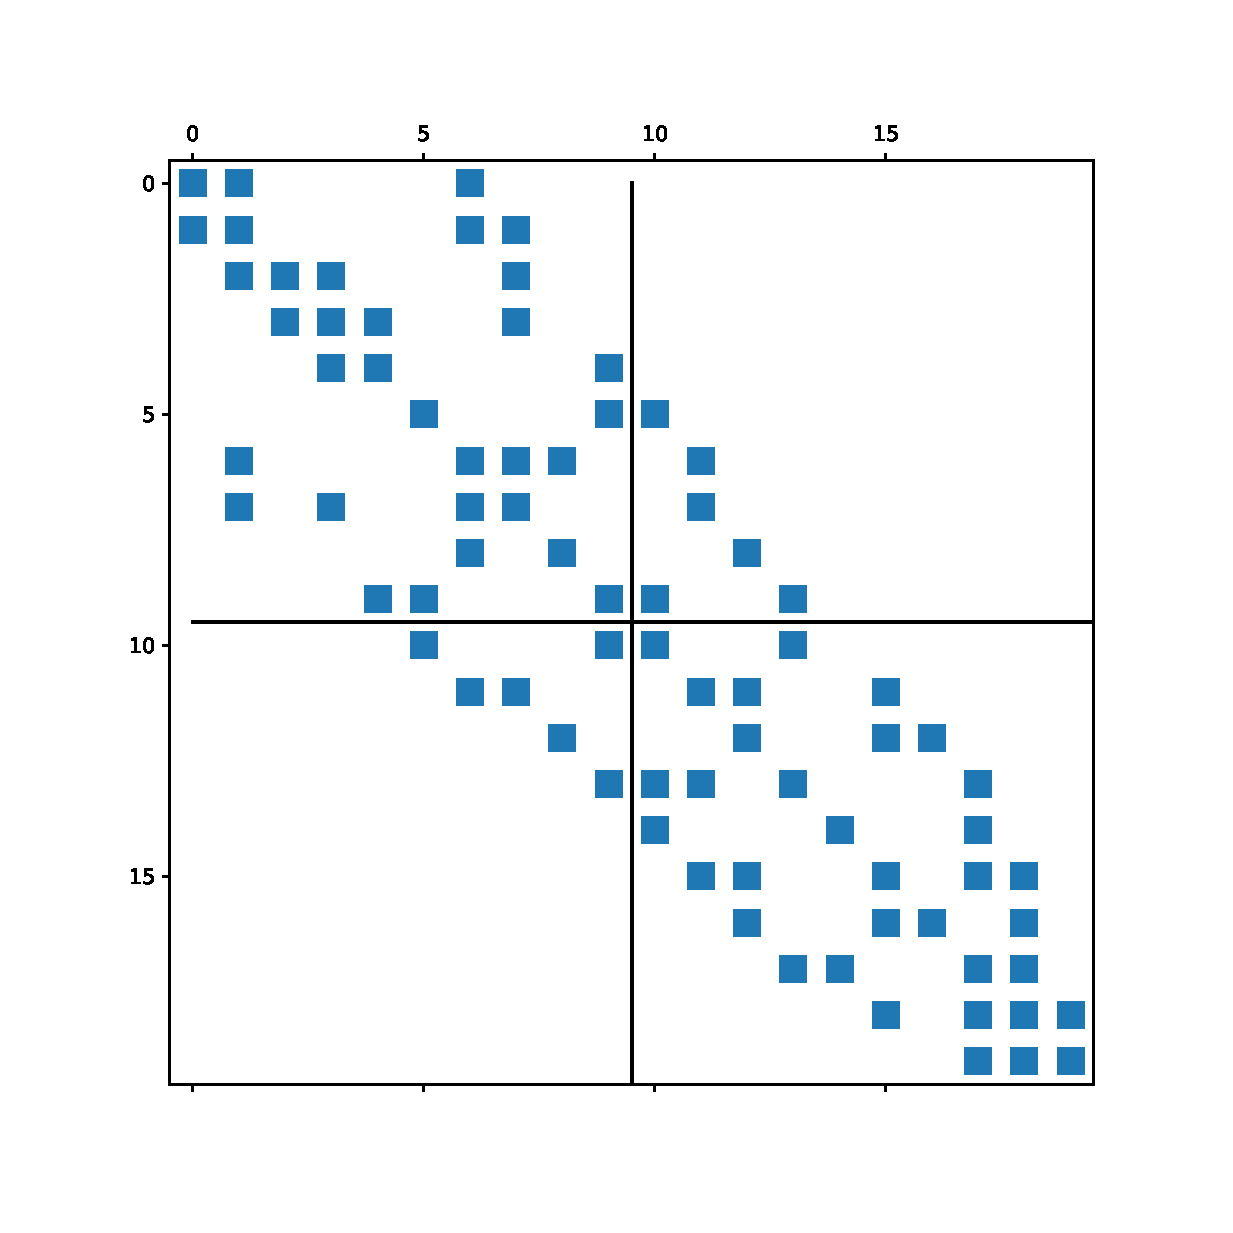
\includegraphics[width=.4\textwidth]{rcm_order_spy.eps} \\
			Unordered & RCM Ordering \\
		\end{tabular}
		\caption{Four ways to partition the disk with equal area.}
		\label{matrix_spy}
	\end{figure}
	
	While the differentiation matrix is unknown beforehand, we do know its sparsity pattern. Each row consists of the weights of the stencil centered at the corresponding point, and only the nearest neighbors are considered. If all of the rows corresponding to these nearest neighbors are allocated to the same process, then the calculation of this row will only need vector values already stored on this process. 
	
	\begin{figure}[ht]
		\centering
		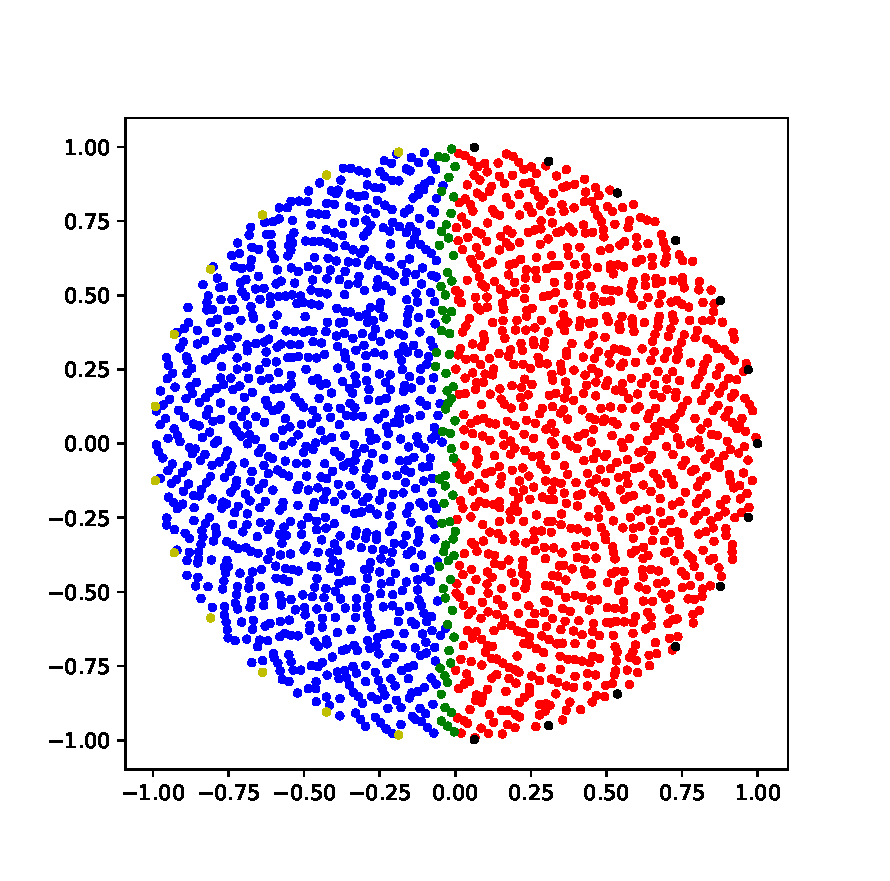
\includegraphics[width=.75\textwidth]{nearest_2proc_disk.eps}
		\caption{Partitioning of the domain }
		\label{nearest_2proc_disk}
	\end{figure}
	
	Suppose that we partition the unit disk along the $y$-axis so that all points on the right are allocated to process one and the rest are allocated to process two. This can be seen in figure \ref{nearest_2proc_disk} where process one is responsible for the red and black points and process two is responsible for the rest. The green points denote points belonging to process two, but who are nearest neighbors to points in process one. Thus, process one will need to know the vector values corresponding to the green points in order to calculate the matrix vector product. 
	
	In this way, the geometric partitioning of the domain is very important for the sparsity pattern of the matrix. In particular, we would like it so that the off-diagonal blocks of the matrix are as sparse as possible. 
	
	\begin{figure}[ht]
		\centering
		\begin{tabular}{cc}
			\includegraphics[width=.4\textwidth]{disk_decomp_strips.eps} & \includegraphics[width=.4\textwidth]{disk_decomp_quad.eps} \\
			Stripes & Quadrants \\
			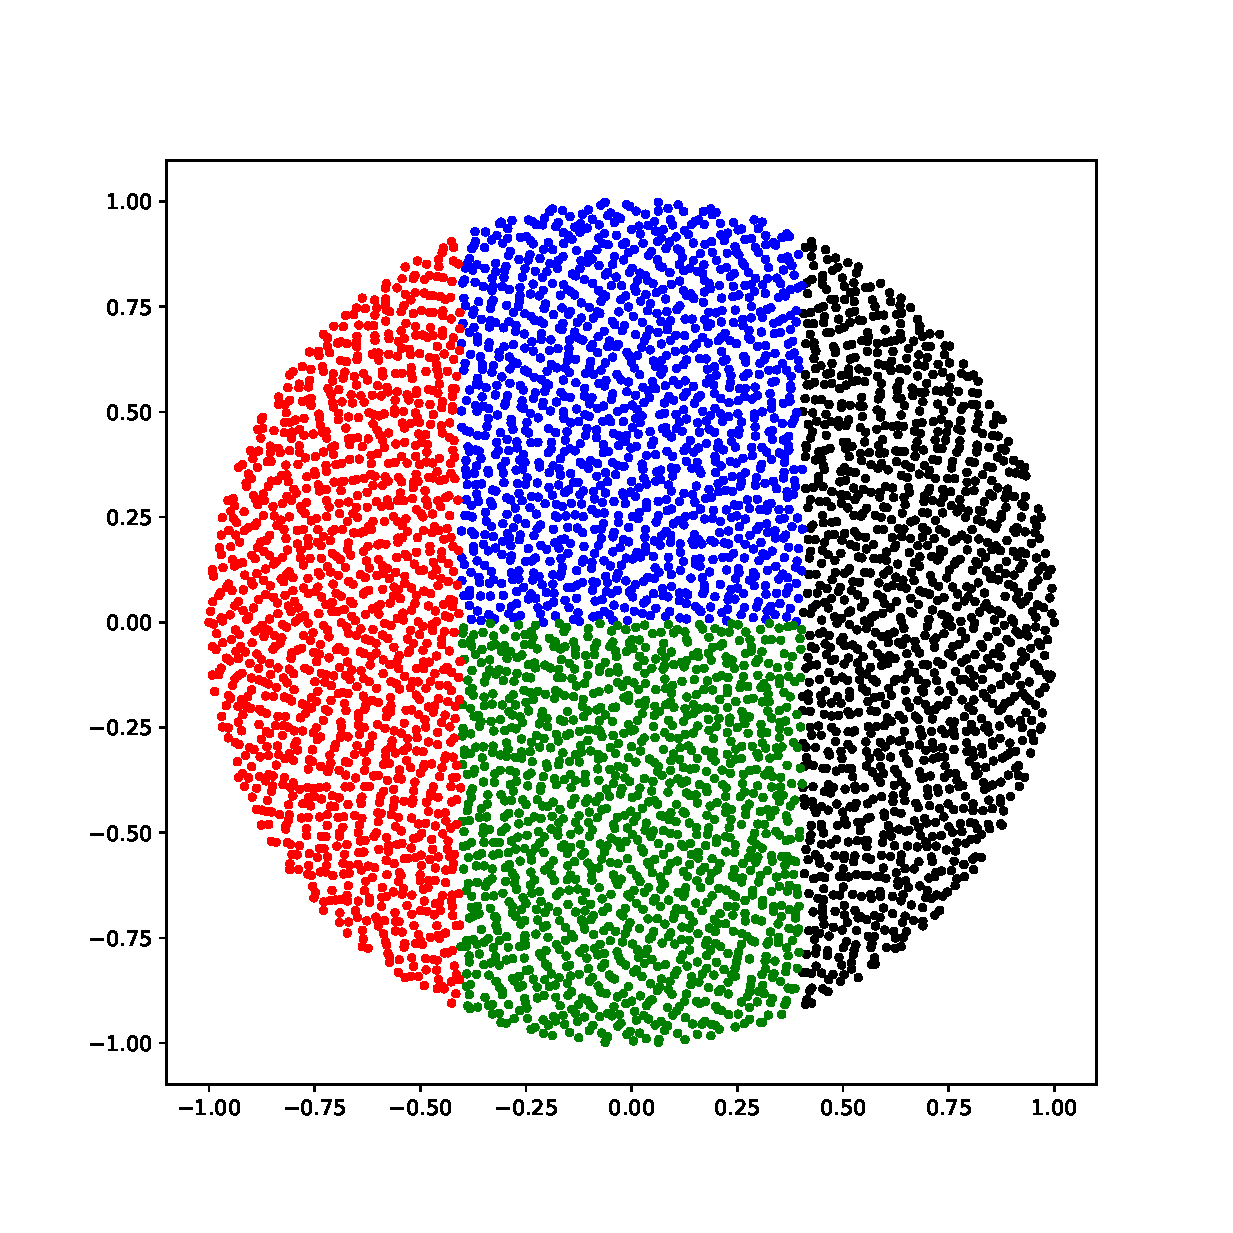
\includegraphics[width=.4\textwidth]{disk_decomp_cake.eps} & \includegraphics[width=.4\textwidth]{disk_decomp_triangle.eps} \\
			Cake-cutting & Triangle-cutting
		\end{tabular}
		\caption{Four ways to partition the disk with equal area.}
		\label{decomp_strategies}
	\end{figure}
 
	 Figure \ref{decomp_strategies} shows four possible geometric partitions of the unit disk into four equal area sections. Given a particular partition it would be advantageous to order the points (and hence the rows and columns of the matrix) so that for each partition the nodes that are shared with a neighboring process are contiguous in memory. The length of the shared boundary between two processes will be proportional to the number of points that need to be shared and thus should be minimized. The number of adjacent processes to a given process will determine how many times communication must be initiated for a given process and should also be minimized. 
	 
	 The Stripes and Quadrants patterns in figure \ref{decomp_strategies} illustrate two extremes between these two constraints. The Stripes pattern attempts to reduce the of neighboring processes while the Quadrants pattern tries to reduce the shared boundaries between processes. In the stripes pattern a given process will need to communicate with at most two other processes but has a shared boundary of about twice the diameter of the disk. In the Quadrants pattern each process has three neighbors but the length of the shared boundary is exactly the diameter of the disk.
	 
	 In MPI the overhead of communicating data between processes is the dominating factor in regards to computation time. In light of this I've decided to go with the Stripes pattern as it is the simplest and involves the fewest number of communications. It also is the easiest to generalize to larger process counts.
	 
\subsection{Iterative Solver}
	The part that I'm struggling with at this point is the choice of iterative solver. Our matrix is not SPD so conjugate gradient (CG) is off the table. My next choice would be to use GMRES but parallelizing GMRES seems too challenging. Donna suggested that I look at BiCGSTAB - a variant of bi-conjugate gradient (BiCG) which is in turn a variant of CG. BiCGSTAB would be parallelizable however in practice it doesn't always converge. In particular I've tested it on a sample problem generated from RBF-FD and it fails to converge. BiCGSTAB is often paired with the incomplete LU (ILU) decomposition as a preconditioner. This seems much more stable and did succeed at solving all of the test problems that I generated, however parallelizing the ILU also looks challenging. 
	
	Your suggestion to transform the system from $D\vec{u} = \vec{f}$ to $D^TD\vec{u} = D^T\vec{f}$ forcing the matrix $D^TD$ to be SPD so that we may use CG looks to be the easiest work around. There are two main disadvantages to this however. The first is that the condition number of $D^TD$ will be much larger than the condition number of $D$ which will significantly lower the maximum size of the system that will still give good numerical solutions to the PDE. The second drawback is that $D^TD$ will be significantly less sparse than $D^T$ making iterations more expensive.
	
	While this solution will be easier than the alternatives, it will still prove challenging. Our matrix will be stored in a compressed format making the formulation of the transpose more complicated.
	
% \bigbreak
\pagebreak
 
\printbibliography

\end{document}
